\documentclass[course=asp]{aspdoc}
\usepackage{graphicx}
\graphicspath{{./Bilder/}}

\newcommand{\theGroup}{team 117} % Beispiel: 42
\newcommand{\theNumber}{502: XTEA} 
\author{Guo, Linfeng\\Gönenc, Hazar \\Özakay, Baris}
\date{Wintersemester 2021/22} 


% Diese Zeile bitte -nicht- aendern.
\title{Gruppe \theGroup{} -- Abgabe zu Aufgabe \theNumber}

\begin{document}
\maketitle



\section{Einleitung}
Im Rahmen unseres Projektes im Fach Aspekte der systemnahen Programmierung bei der Spieleentwicklung war es unsere Aufgabe, ein Ver- und Entschlüsselungsalgorithmus XTea in Assemblercode zu programmieren. Diese Aufgabe lässt sich in folgende Bereiche aufteilen: Konzeption, die Funktionsweise des XTEA Algorithmus und Verfahren für die Optimierung des Algorithmus, verstehen; der XTEA Algorithmus in Assemblercode zu implementieren …(Aufgabe von Baris). Die Bearbeitung dieser Teilbereiche wird im Folgenden Beschrieben.  \\In der Grafik zu sehen ist ein Beispiel für die Ver- und Entschlüsselung mit dem XTEA Algorithmus.  

\newpage
\section{Lösungsansatz}
\subsection*{2.1.Feistelchiffre }
Der XTEA Algorithmus ist ein Verschlüsselungsalgorithmus, welche auf die Struktur von Feistelchiffre basiert ist. Feistelchiffre ist eine Struktur, die für symmetrische Verschlüsselung verwendet wird. Unter symmetrische Verschlüsselung ist zu verstehen, dass für die Ver- und Entschlüsselung nur ein Key verwendet wird. Wir würden daher erstmal mit Feistelchiffre, die grundstruktur der symmetrische Verschlüsselung, eingehen.\\
Feistelchiffre lässt sich in vier Schritten aufteilen. Zuerst hat man ein Klartextblock mit der Nachricht, weche meist 8 Bytes ist, und teilt diese in zwei gleich große Bl\"ocke L0 und R0, die 4 Bytes entsprechen auf.

\begin{table}[H]
\centering 
    \begin{tabular}{|l|l|l|l|l|l|l|l|}
        \hline
        B & E & I & S & P & I & E & L   \\
        \hline
    \end{tabular}
    \caption{Nachricht}
\end{table}

\begin{table}[H]
\centering 
    \begin{tabular}{|l|l|l|l|l|l|l|l|}
        \hline
        42 & 45 & 49 & 53 & 50 & 49 & 25 & 4C   \\
        \hline
    \end{tabular}
    \caption{Nachricht in Hex Code}
\end{table}



\begin{table}[H]
    
    \begin{minipage}{.5\linewidth}
      
      \centering
        \begin{tabular}{|l|l|l|l|}
		\hline
            42 & 45 & 49 & 53   \\
		\hline
        \end{tabular}

	\caption{L0}
    \end{minipage}%
    \begin{minipage}{.5\linewidth}
    
 \centering
        
        \begin{tabular}{|l|l|l|l|}
           \hline
		 50 & 49 & 25 & 4C   \\
		\hline
        \end{tabular}
\caption{R0} 
    \end{minipage}
\end{table}
Danach findet die eigentliche Verschlüsselung statt. Man führt die Verschlüsselungsfunktion mit der Schlüssel,der ebenfalls 4 Byte entspricht, auf R0 aus. Die Funktion bei Feistelchiffre ist allerdings undefiniert, da Feistelchiffre nur die Struktur anbietet. Der Wert der durch die Funktion ergibt, wird anschließend mit dem linken Teil durch die XOR- Operation eingefangen. So ergibt sich das neue R1. Die ursprüngliche R0 wird dann zu L1. Nach jeder Verschlüsselung wird die Position vom linken und dem rechten Block getauscht, sowie oben beschrieben wird.\\
Die Entschlüsselung funktioniert im Prinzip genau wie die Verschlüsselung. Nur mit dem Unterschied, dass man die Position vom linken und rechten Teil tauscht. Also wird Ln+1 in die Funktion mit demselben Key eingesetzt und das Ergebnis wird dann mit Rn+1 per XOR abgebildet. Der Wert wird dann zu Rn und Ln+1 wird zu Ln.  

\begin{figure}[h]
\centering
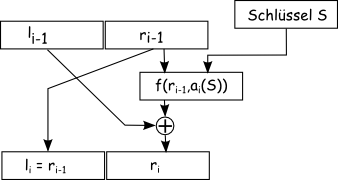
\includegraphics[scale = 0.4]{feistel.png}
\caption{Feistelchiffre}
\end{figure}
\newpage


\subsection*{2.2.XTEA}
Die Aufgabe des Projekts liegt darin den XTEA Algorithmus sowohl in C als auch in Assembler zu implmentieren. Für die Implementierung der XTEA Algorithmus soll man zunächst wissen wie XTEA überhaupt funktioniert. \\
Das Verfahren von XTea ist auf Feistelchiffre basiert. Der eingelesene Wert, welcher 8 Byte entspricht, wird in zwei Blocken aufgeteilt, V1 und V2. Für XTea brauchen wir zusätzlich noch eine weitere Variable s, die Summe, die immer nach der Verschlüsselung Vvon 1 mit der magischen Zahl ${\delta}$ addiert wird. ${\delta}$ lässt sich aus der Formel:
\begin{equation}
     \delta  =   \lfloor ( \surd 5 -1)  \cdot  2^{31} \rfloor
\end{equation}
berechnen. Jede Runde findet eine doppelte Verschlüsselung statt. \\
Zuerst ist die Verschlüsselung von V1. Da wird V2 in zwei Blöcken geshiftet. Block 1 ist V2 << 4 und Block ist V2 >>5. Die zwei Blöcken werden per XOR zu einem neuen Wert abgebildet und zu V2 addiert. Danach wird V2 mit der Summe von s, welche am Anfang Null ist, und der Schlüssel, dessen Index aus der Variable s Modulo drei ergibt, per XOR abgebildet. Das Ergebnis wird zum Schluss auf V1 addiert. \\
Zur veranschaulichung nehmen wir wieder das Beispielwort "BEISPIEL". Und teilen dieses Wort in V1 und V2 auf. 
\begin{table}[H]
    
    \begin{minipage}{.5\linewidth}
      
      \centering
        \begin{tabular}{|l|l|l|l|}
		\hline
            42 & 45 & 49 & 53   \\
		\hline
        \end{tabular}

	\caption{V1}
    \end{minipage}%
    \begin{minipage}{.5\linewidth}
    
 \centering
        
        \begin{tabular}{|l|l|l|l|}
           \hline
		 50 & 49 & 25 & 4C   \\
		\hline
        \end{tabular}
\caption{V2} 
    \end{minipage}
\end{table}
 
Anschließend follgt das Shiften von V2. Die XOR Operation wird danach an den beiden Blöcken ausgeführt.
\begin{table}[H]
    
    \begin{minipage}{.5\linewidth}
      
      \centering
        \begin{tabular}{|l|l|l|l|}
		\hline
            04 & 92 & 54 & C0   \\
		\hline
        \end{tabular}

	\caption{V2 << 4}
    \end{minipage}%
    \begin{minipage}{.5\linewidth}
    
 \centering
        
        \begin{tabular}{|l|l|l|l|}
           \hline
		 02 & 82 & 49 & 2A   \\
		\hline
        \end{tabular}
\caption{V2 >> 5} 
    \end{minipage}
\end{table}

\begin{table}[H]
\centering 
    \begin{tabular}{|l|l|l|l|}
        \hline
        06 & 10 & 1d & es    \\
        \hline
    \end{tabular}
    \caption{V2 << 4 $\oplus$ V2 >> 5}
\end{table}
Das Ergebnis wieder auf V2 addiert und 
  








Die Variable s wird jetzt um die magische Zahl erhöht. Für V2 funktioniert die Verschlüsselung ähnlich wie bei V1. Wir teilen V1 in zwei Hälften auf und genau sowie bei V1, werden die zwei Hälften per XOR zu einem neuen Wert dargestellt und zu V2 addiert. V2 verschlüsselt sich dann per XOR mit der Summe von s und der Schlüssel, dessen Index jetzt aus s shift 11 Modulo 3 besteht. 

Die Vorgehensweise beide Verfahren haben Gemeinsamkeiten und Unterschiede. Da XTea auf Feistelchiffre basiert ist, erkennt man auch das symmetrische Verschlüsselungsverfahren bei ihm, d.h. für die Ver- und Entschlüsselung der Nachricht wird denselben Schlüssel verwendet. Bei beidem wird am Anfang der Verschlüsselung die zu verschlüsselnden Daten in zwei Blöcken aufgeteilt und das Verschlüsselungsprozess kann zu mehreren Runden dauern. Die Länge der zu verschlüsselnden Daten muss immer ein Vielfaches der Block-länge sein. Auch das Benutzen von XOR kann man bei beiden Verfahren finden. 
\begin{figure}[h]
\centering
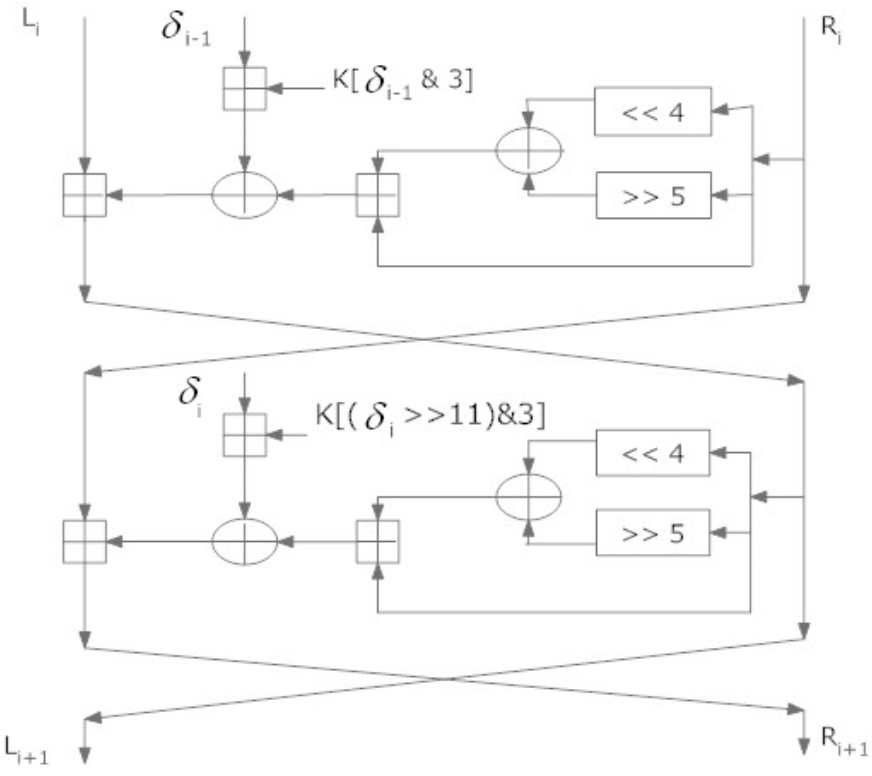
\includegraphics[scale = 0.55]{XTEA.png}
\caption{XTEA}
\end{figure}
\newpage




\newpage
\subsection*{2.3.Unterschiede und Gemeinsamkeiten zwischen XTEA und Feistelchiffre}
Es gibt aber auch Unterschiede zwischen beiden Verfahren. Bei XTea findet jede Runde eine doppelte Verschlüsselung statt, was bei Feistelchiffre nicht zu finden ist. Außerdem gibt es bei XTea eine weitere Variable s und die magische Zahl, die bei der Verschlüsselung eine wichtige Rolle spielen. In XTea wird die XOR Operation öfters ausgeführt und zudem verwendet XTea auch das Shiften. Feistelchiffre arbeitet hingegen mit eine Verschlüsselungsfunktion. Nach jedem Runde der Verschlüsselung werden die Position von den zwei Blöcken getauscht, dies kommt bei XTea allerdings nicht vor. \\
Zusammengefasst lässt sich sagen, dass sowohl XTea als auch Feistelchiffre die Voraussetzung für symmetrische Verschlüsselung erfüllen. Bei beidem ist die Länge der zu verschlüsselnden Daten ein Vielfaches der Block-länge. Beide Verfahren teilen die Nachricht für die Verschlüsselung in zwei Blöcken auf, dennoch ist die Key-Schedule bei XTea komplexer ist, im Vergleich zu Feistelchiffre.  
\subsection*{2.4.Padding}


%%test
\newpage
% TODO: Je nach Aufgabenstellung einen der Begriffe wählen
\section{Korrektheit/Genauigkeit}
\subsection*{I/O-Operationen in C}
\subsection*{Implementierung in C}
\subsection*{Implementierung in Assemblercode}
\newpage

\section{Performanzanalyse}
\newpage

\section{Zusammenfassung und Ausblick}

\newpage
% TODO: Fuegen Sie Ihre Quellen der Datei Ausarbeitung.bib hinzu
% Referenzieren Sie diese dann mit \cite{}.
% Beispiel: CR2 ist ein Register der x86-Architektur~\cite{intel2017man}.

%%TODO
\bibliographystyle{plain}
\bibliography{Ausarbeitung}{}

\end{document}
